% Source: Code/ML_overlay/ir_rgb_registration/paper/ml_overlay_report_materials/ir_rgb_registration_report/figures/fig_bilinear_sampling.tex
\documentclass[tikz,border=10pt]{standalone}
\usepackage{tikz}
\usetikzlibrary{arrows.meta,positioning,calc}

\definecolor{garnet}{RGB}{115,0,10}
\definecolor{rose}{RGB}{204,46,64}
\definecolor{atlantic}{RGB}{70,106,159}
\definecolor{congaree}{RGB}{31,65,77}
\definecolor{black90}{RGB}{54,54,54}
\definecolor{black50}{RGB}{162,162,162}

\begin{document}
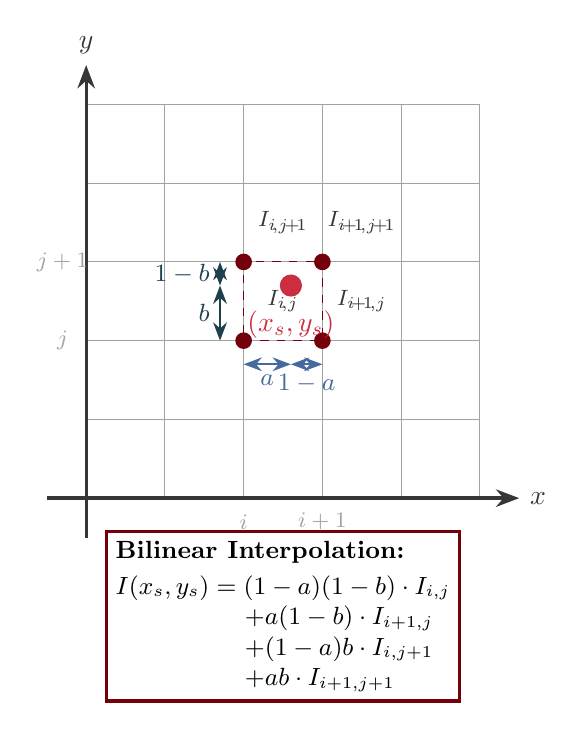
\begin{tikzpicture}[>=Stealth]

    % Grid
    \draw[black50, thin] (0,0) grid (5,5);

    % Four neighboring pixels
    \foreach \x/\y/\label in {2/2/I_{i\!,j}, 3/2/I_{i\!+\!1\!,j}, 2/3/I_{i\!,j\!+\!1}, 3/3/I_{i\!+\!1\!,j\!+\!1}} {
        \fill[garnet] (\x,\y) circle (3pt);
        \node[font=\footnotesize, black90] at (\x+0.5,\y+0.5) {$\label$};
    }

    % Sample point
    \fill[rose] (2.6,2.7) circle (4pt);
    \node[rose, font=\bfseries] at (2.6,2.2) {$(x_s, y_s)$};

    % Distance annotations
    \draw[<->, atlantic, thick] (2,1.7) -- (2.6,1.7) node[midway, below, font=\small] {$a$};
    \draw[<->, atlantic, thick] (2.6,1.7) -- (3,1.7) node[midway, below, font=\small] {$1-a$};

    \draw[<->, congaree, thick] (1.7,2) -- (1.7,2.7) node[midway, left, font=\small] {$b$};
    \draw[<->, congaree, thick] (1.7,2.7) -- (1.7,3) node[midway, left, font=\small] {$1-b$};

    % Reference lines
    \draw[garnet, dashed] (2,2) -- (3,2) -- (3,3) -- (2,3) -- cycle;

    % Axes
    \draw[->, very thick, black90] (-0.5,0) -- (5.5,0) node[right] {$x$};
    \draw[->, very thick, black90] (0,-0.5) -- (0,5.5) node[above] {$y$};

    % Formula box
    \node[draw=garnet, very thick, fill=white, align=left, font=\small] at (2.5,-1.5) {
        \textbf{Bilinear Interpolation:} \\[2pt]
        $I(x_s, y_s) = (1-a)(1-b) \cdot I_{i,j}$ \\
        \phantom{$I(x_s, y_s) =$} $+ a(1-b) \cdot I_{i+1,j}$ \\
        \phantom{$I(x_s, y_s) =$} $+ (1-a)b \cdot I_{i,j+1}$ \\
        \phantom{$I(x_s, y_s) =$} $+ ab \cdot I_{i+1,j+1}$
    };

    % Coordinate labels
    \node[font=\footnotesize, black50] at (2,-0.3) {$i$};
    \node[font=\footnotesize, black50] at (3,-0.3) {$i+1$};
    \node[font=\footnotesize, black50] at (-0.3,2) {$j$};
    \node[font=\footnotesize, black50] at (-0.3,3) {$j+1$};

\end{tikzpicture}
\end{document}
